\documentclass[a4paper,12pt]{article}
\usepackage{geometry}
\usepackage{wrapfig}
\geometry{
      a4paper,
      total={170mm,257mm},
      left=10mm,
      right=10mm,
      top=20mm,
}
\usepackage{titlesec}
\titlelabel{\thetitle.\quad}
\usepackage{cmap}
\usepackage{mathtext}
\usepackage{parskip}
\usepackage[T2A]{fontenc}
\usepackage[utf8]{inputenc}
\usepackage[english,russian]{babel}
\usepackage{amsmath,amsfonts,amssymb,amsthm,mathtools}
\usepackage{icomma}
\usepackage{euscript}
\usepackage{mathrsfs}
\usepackage{gensymb}
\usepackage{graphicx}
\usepackage{setspace}
\usepackage{tabularx}
\usepackage{longtable}
\usepackage{icomma}
\usepackage{euscript}
\usepackage{float}
\usepackage{cutwin}
\usepackage{adjustbox}
\usepackage{dashbox}
\usepackage[normalem]{ulem}
\usepackage[babel=true]{microtype}
\RequirePackage[T1]{fontenc}
\usepackage{amsmath,amsfonts,amssymb,amsthm,mathrsfs,mathtools}
\usepackage{xcolor}
\usepackage{enumitem}
\usepackage{xpatch}
\usepackage{cancel}
\usepackage{upgreek}
\usepackage{lipsum}
\usepackage[version=4]{mhchem}
\usepackage{multirow}
\usepackage{stackengine}
\usepackage{tikz}
\usepackage{hyperref}
\hypersetup{colorlinks=true,urlcolor=blue}
\usetikzlibrary{positioning}
\usepackage{titletoc}
\usepackage{chngcntr}
\usepackage{fancyhdr}
\usepackage{makecell}
\usepackage{indentfirst}
\usepackage{tocloft}
\usepackage{soul}
\usepackage[stable]{footmisc}
\setlength{\parskip}{1ex}
\setlength{\parindent}{0ex}
\usepackage{subfig}
\usepackage{comment}
\title{Полный анализ функции}\begin{document}

\maketitle
\renewcommand{\abstractname}{Введение}\begin{abstract}Данный документ содержит полный анализ функции с разложением в ряд Тейлора, построением графика и взятием полной производной.\end{abstract}
\section*{Исходная функция}

$f(x, , z, y) = {{\ln{({x} + {z})}} \cdot {({3} + {y})}}$

\section{Взятие 1-ой производной по x}

$ f(x) = {{\ln{({x} + {z})}} \cdot {({3} + {y})}}$

Кто бы мог подумать что:

${({{\ln{({x} + {z})}} \cdot {({3} + {y})}})}^{'} = {({\ln{({x} + {z})}})}^{'}\cdot {{3} + {y}} + {\ln{({x} + {z})}}\cdot {({{3} + {y}})}^{'}$

Можно убедиться, что:

${({{3} + {y}})}^{'} = {({3})}^{'} + {({y})}^{'}$

Заметим, что:

${({y})}^{'} = 0$

Не требует дальнейших комментариев:

${({3})}^{'} = 0$

Заметим, что:

${({\ln{({x} + {z})}})}^{'} = {{{({{x} + {z}})}^{'} } \over {{{x} + {z}}}}$

Кто бы мог подумать что:

${({{x} + {z}})}^{'} = {({x})}^{'} + {({z})}^{'}$

Нетрудно заметить:

${({z})}^{'} = 0$

Увидим, что:

${({x})}^{'} = 1$

Получаем:

$ f^{(1)}(x) = {{{{({1} + {0})} \over {({x} + {z})}} \cdot {({3} + {y})}} + {{\ln{({x} + {z})}} \cdot {({0} + {0})}}}$

\section{Упрощение}

${{{{({1} + {0})} \over {({x} + {z})}} \cdot {({3} + {y})}} + {{\ln{({x} + {z})}} \cdot {({0} + {0})}}} = {{{1} \over {({x} + {z})}} \cdot {({3} + {y})}}$
\section{Вычисление значения функции в точке}

$ f(100) = 32.5777 $
\section{Вычисление производной функции в точке}

$ f^{'}(5) = 0.7 $
\section{Разложение данной функции в ряд Тейлора}

${{\ln{({x} + {z})}} \cdot {({3} + {y})}} =  11.2661 + \frac{1.4}{1}\cdot x^1 - \frac{0.28}{2}\cdot x^2 + \frac{0.112}{6}\cdot x^3 - \frac{0.0672}{24}\cdot x^4 + \frac{0.05376}{120}\cdot x^5 - \frac{0.05376}{720}\cdot x^6 + \frac{0.064512}{5040}\cdot x^7 + o(x^7) $
\section{Взятие полной производной}

$F(x, , z, y) = \sqrt{({{{1} \over {({x} + {z})}} \cdot {({3} + {y})}} \cdot \Delta x)^2 + ({0} \cdot \Delta )^2 + ({{{1} \over {({x} + {z})}} \cdot {({3} + {y})}} \cdot \Delta z)^2 + ({\ln{({x} + {z})}} \cdot \Delta y)^2} $

\section{Уравнение касательной функции в точке x = 2}

g(x) = $1 \cdot  x + 11.6214 $
\section{График функции и касательной к ней}


\begin{figure}[ht]
\center
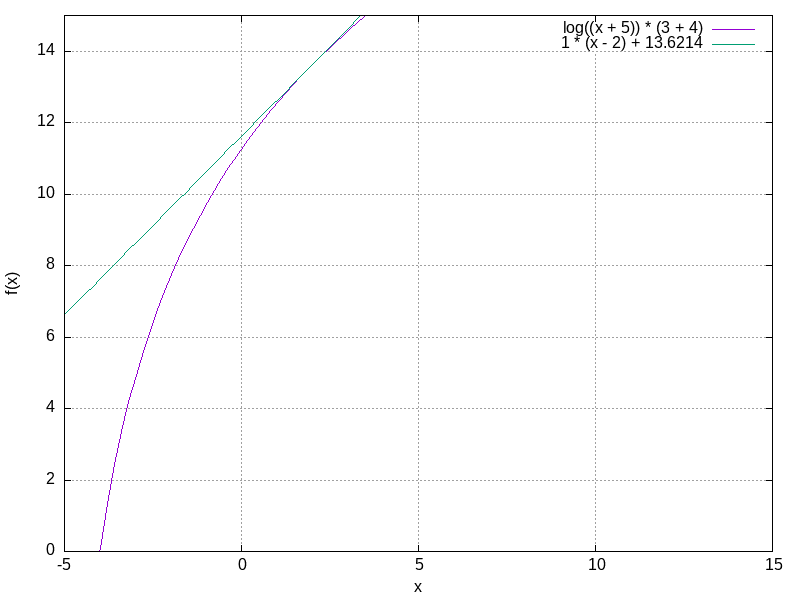
\includegraphics[scale=0.65]{graph.png}
\end{figure}
\end{document}